\chapter{实验与结果分析}

\section{基于强化学习的资源调度器}
图\ref{fig:rl}显示了我们想实现的基于强化学习的资源调度器的基本框架,图\ref{fig:overview}显示了更具体的实验环境,智能体将通过观察环境的状态和所执行动作带来的奖励,学习如何分配资源给延迟敏感型任务和批处理任务。智能体在每一个调度周期开始前做出资源分配决策,在新的调度周期开始时,智能体观察环境状态并做出新的资源分配决策。


\subsection{状态空间}
本问题中,环境的状态即为服务器上各种资源的利用率,和延迟敏感型任务及批处理任务的运行状态。实验中,智能体所能观察到的状态参数包括以下三种:
\begin{enumerate}
  \item 延迟敏感型任务在即将开始的调度周期中的负载;
  \item 上一个调度周期内,各个任务对计算核心的利用率;
  \item 上一个调度周期内,各个任务对动态随机存储访问带宽的利用率;
\end{enumerate}

\vspace{1em}
第一个参数,即将开始的周期内的负载强度,可以通过当前延迟敏感型任务的连接总数获得,或通过前几段调度周期记录的负载强度估计获得。通过对当前调度周期负载强度的估计,智能体可以初步判断所需的计算核心与缓存资源。

第二组和第三组参数帮助智能体了解前一周期分配的资源利用的情况。当前调度周期的负载强度不能描述负载的全部特征:对于对象缓存服务来说,操作包括读取和写入。当写入为主要请求类型时,仅仅提高末级高速缓存并不能有效提高写入性能;当读取为主要负载类型时,延迟敏感型任务可能对末级高速缓存的容量更加敏感。当负载的各操作类型比例变化时,延迟敏感型对所获得的资源利用情况之间将存在差异。因此,我们希望通过在环境状态中加入上一调度周期的资源利用率的信息,帮助智能体捕获不同负载类型组合对资源需求的差异,以做出更优化的决策。

% 通过判断两个调度周期负载的强度,智能体可以判断是否增加或减少分配给延迟处理任务的资源,例如两个调度周期内的负载强度相同或仅有很小的变化,智能体可以直接返回上一次资源分配的结果,并有很大信心相信此分配可以保证延迟敏感型任务的服务质量。
% 例如第三和第四个参数可以帮助智能体了解上一次做出的决策对混合执行的任务的计算造成的影响,并随之调整。例如上一次做出的资源分配造成延迟敏感型任务的计算核心利用率低下,大量处理器时间处于空闲状态,若本次调度周期内的负载变化不大,则可以尝试适当降低分配给延迟敏感型任务的计算核心,以提高批处理任务的计算性能和系统资源利用率。第五和第六个参数,可以帮助智能体了解上次资源分配对随机动态存储访问带宽压力的影响。例如,若批处理任务占用大量的内存访问带宽,智能体则需要学会判断是否末级高速缓存成为了批处理任务的性能瓶颈,延迟敏感型任务在此时对末级高速缓存的容量是否敏感以便扩大批处理任务的缓存容量,以及若不能提高批处理任务的缓存容量,是否需要减小运行批处理任务的核心数目以减小其访存带宽占用,避免影响延迟敏感型任务对内存的访问。基于前面参数的信息,智能体结合第七和第八个参数可以输出此调度周期的资源分配方案。


\subsection{动作空间}
智能体的动作空间即为输出当前调度周期内延迟敏感型任务和批处理任务各自可用的计算核心数和末级高速缓存容量。实验中的服务器上共有十个物理核心(二十个逻辑核心),分配粒度为二十分之一共享末级高速缓存。

当动作空间过大时,强化学习算法需要大量样本,收敛缓慢。通过具体问题中的条件来限制动作空间大小可有效加快学习算法收敛的速度。由于同一物理核心上运行的线程将共享第一和第二级缓存,且其上的干扰无法控制,因此设置计算核心调度的粒度为单个物理核心。延迟敏感型任务在最低负载时运行的需要的最少资源,以及分析应用对各个资源分配的敏感程度并合理设置资源分配粒度也可以有效减小动作空间。
\begin{figure}[!h]
  \centering
  \begin{subfigure}{0.47\textwidth}
    \centering
    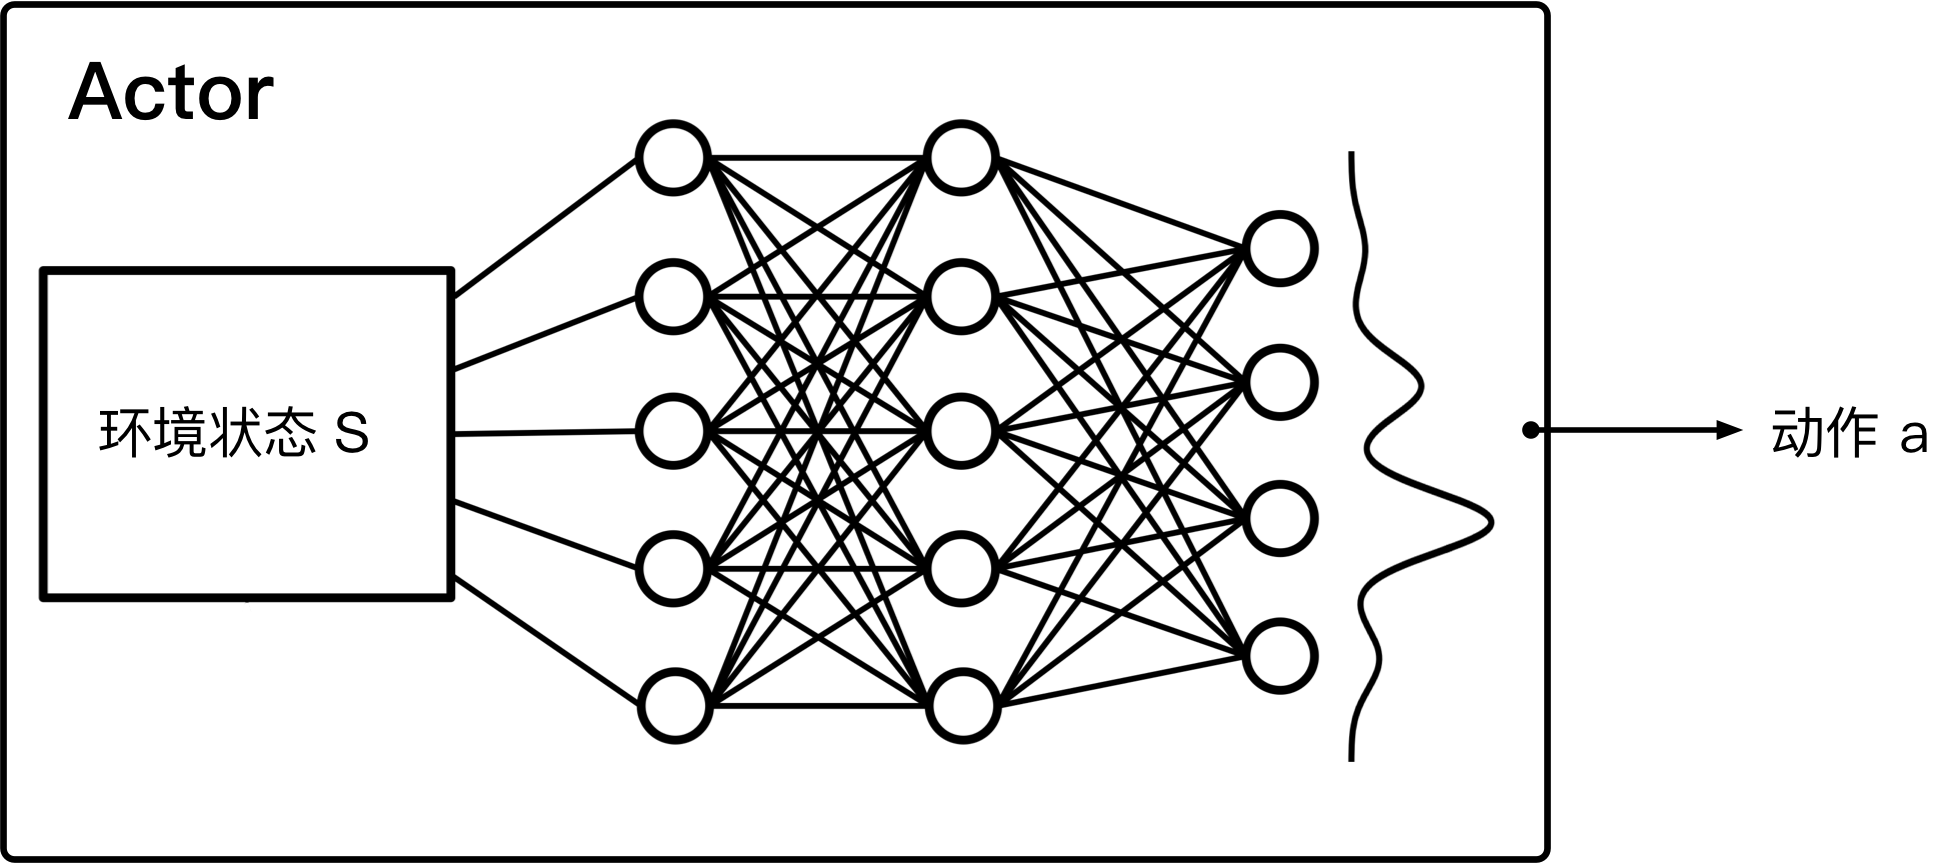
\includegraphics[width=1\linewidth]{result/actor.png}
    \caption{Actor选择动作}
  \end{subfigure}
  % \hspace{1em}
  \begin{subfigure}{0.49\textwidth}
    \centering
    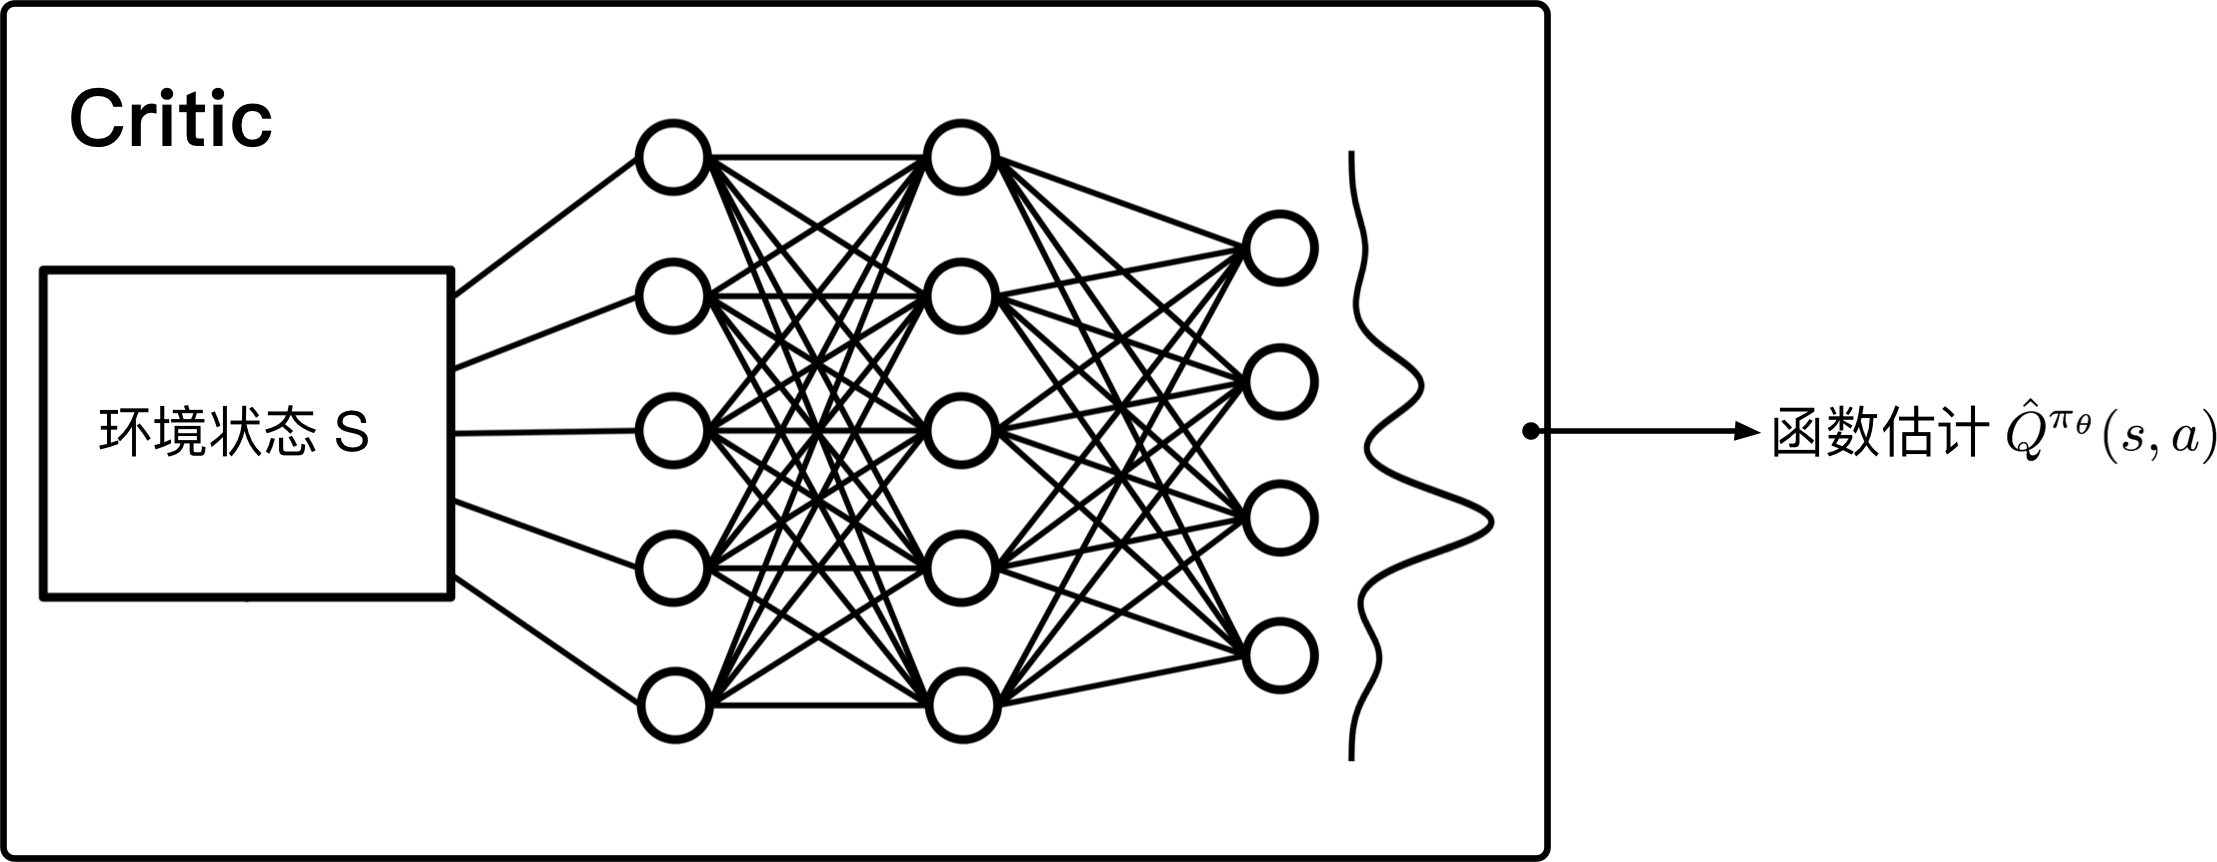
\includegraphics[width=1\linewidth]{result/critic.png}
    \caption{Critic输出值函数}
  \end{subfigure}
  \captionof{figure}{强化学习网络}
  \label{fig:actor_critic}
\end{figure}

% todo the actual action space
\subsection{奖赏信号结构}
智能体的优化目标包括两部分,首先要保证延迟敏感型任务不违反其给定的服务质量要求,其次,智能体需要尝试提高服务器资源的利用率。因此,奖赏信号不但应该与延迟敏感型任务的服务质量相关,还应同时反应服务器资源的利用率情况。若假设批处理任务可以充分利用所有分配的资源,此时智能体的优化目标可等价为尽量减少分配给延迟敏感型任务的资源。

奖赏信号设计的难点在于无法通过预先设置一个函数判断是否智能体分配分配给延迟敏感型任务的资源足够少。如果这样的函数易于设计,我们也不需要通过强化学习来试图解决数据中心的资源调度问题。一个替代的指标是在执行智能体给出的资源分配方案后,采样测得的延迟敏感型任务的服务质量。例如服务质量被定义为延迟时,如果测得的延迟远小于服务质量要求,我们可以判断智能体给延迟敏感型任务分配了过多的资源。如果在为延迟敏感型任务过多分配资源时,智能体获得奖励,智能体将倾向于过多分配资源保证奖励的获得。与此相同,我们不希望出现的情况还有智能体分配给延迟敏感型任务的资源太小以至于其违反服务质量要求。值得注意的是,由于资源分配的粒度和延迟敏感型任务对资源分配的敏感性,一些情况下无法使得服务质量处于我们设定的区间,然而智能体的行为是正确的,不应该被惩罚。
因此,我们设定奖励函数如下,当延迟敏感型任务处在我们设定的合理区间内时,智能体获得正的奖赏信号;当测得的服务质量违反了服务质量要求,返回给智能体负的奖赏信号;当测得服务质量高于预期时,给与智能体零的反馈信号。智能体获得的奖励r(t)如式\ref{eq:reward}所示。对象缓存服务Memcached的服务质量要求为九十分位延迟$p^{\operatorname{90th}}_t$小于10毫秒。

\begin{equation}
	r(t) = \begin{cases} 
      \,\,\,0 & p^{\operatorname{90th}}_t< 5 \\
      \,\,\,1 & 5 \le p^{\operatorname{90th}}_t < 10 \\
      -1 & 10 \leq p^{\operatorname{90th}}_t
   \end{cases}
   \label{eq:reward}
\end{equation}


\section{网络设计}
参考David Silver等人使用的算法\cite{mnih2015human},实验的神经网络结构设计如图\ref{fig:actor_critic}所示(不代表真实神经网络层数和神经元数量)。我们采用实现的Actor和Critic使用相同的底层网络结构。Actor-Critc算法本身通过采样的方式估计状态转移,因此网络在输入环境状态后,输出分别采取各个动作后可能转移到的环境状态的状态值期望;Actor通过此输出选择最优策略。

我们通过我们还采用经验回放池以减少连续动作之间的关联性造成的训练低效,同时提高数据利用率。另外,为了保证智能体足够探索可能的环境空间,Actor通过$\epsilon$-贪婪算法($\epsilon$ -greedy)选择执行动作\cite{sutton1998reinforcement},即通过连续型均匀分布在$[0, 1]$间取值大于\epsilon时,Actor将随机选择动作执行,反之Actor将根据Critic的评价选择最优的动作。$\epsilon$将随着训练过程的增加逐渐减小,Actor的行为也将由更倾向于探索环境逐渐变为更倾向于执行最优动作。



\begin{algorithm}
% \begin{algorithm}[H] % 强制定位
\caption{强化学习网络训练算法}
\label{algo:merge_sort}
\begin{algorithmic} %每行显示行号 [1]
\State 初始化训练次数为$T$,Actor更新间隔为$C$
\State 初始化经验回访池$D$,设置大小为$N$,每次取样个数为$M$
\State 初始化状态序列 $S$\gets $\{s_1\}$
\State 初始化Actor网络$Q$,参数$\theta$设为随机生成的参数$\theta'$
\State 初始化Critc网络$\hat Q$,参数$\hat\theta$设为上一步生成的参数$\theta'$

\For {$t = 1... T$}
\If{随机选择动作} \Comment{随机选择动作的概率为$\epsilon$}
\State	$a_t \gets $ 随机动作
\Else
\State	$a_t \gets \underset{a}{\mathrm{argmax}}\,Q(s_t,a)$
\EndIf
\State 减小$\epsilon$,执行动作$a_t$,观察到奖励$r_t$,环境状态$s_{t+1}$
\State 在经验回放池$D$中记录经验$(s_t, a_t, r_t, s_{t+1})$
\State 从经验回放池中随机取样$M$个经验
\For {经验$(s_j, a_j, r_j, s_{j+1})$}
\State $y_j \gets r_j + \gamma\,\underset{a'}{\operatorname{argmax}}Q(s_{j+i}, a')$
\State 对Critic网络参数$\hat\theta$通过梯度下降方法更新,损失函数为$(y_j - \hat Q(s_j, a_j))^2$
\EndFor
\State 每经过$C$次迭代,$\theta \gets \hat\theta$
\EndFor

\end{algorithmic}
\end{algorithm}

\section{实验结果}
我们统计智能体做出的最新一百个动作所获得的平均奖赏来监控智能体训练的过程,平均奖赏最终稳定在0.6附近波动。在智能体的资源分配策略稳定后,截取到如图\ref{fig:run_example}所示的智能体在一段时间内的资源分配决策。可以看到智能体对于计算核心的分配基本上跟随延迟敏感型任务的负载强度变化,且延迟敏感型任务的延迟基本保持在我们确定的目标区间1至10毫秒内。

值得注意的是,在末端负载强度较低(低于0.4时),智能体对计算核心的分配出现剧烈抖动,且基本与负载强度不相当。在延迟随负载强度的变化中可以看到,此段时间内资源分配的变化并没有显著引起延迟敏感型任务的服务质量变化,且延迟均基于我们设置的延迟目标区间的下限1ms至下。我们认为,在负载强度较低时,一方面延迟敏感型任务对于计算资源的增加并不敏感,因此具有几乎相同的服务质量;另一一方面对于低负载,以物理核心为资源分配粒度过于粗糙,以至于在临界情况,减少一个物理核心将违反服务质量要求,而增加核心服务质量又远高于我们的要求。

正是由于这种不敏感,使得智能体在当前的奖励信号设计之下,无法通过学习来区分此种情况下各种资源分配的优劣——因为在这些资源分配中,智能体获得的都是零的奖励。

因为对象缓存任务对缓存容量不敏感(见3.3节资源需求分析),同样的情况也发生在智能体对末级高速缓存的分配上。可以看到末级高速缓存的大小的确对延迟敏感型任务的服务性能存在影响,然而不同的分配方案对延迟的影响均不大。延迟的升高或降低都保持在我们设计的目标区间内。同低负载时任务对计算核心的不敏感一样,我们需要改进奖赏信号的设计以使得智能体有能力区分不同的分配策略,进而保证智能体学习到最优的资源分配策略。

在低负载情况时以物理核心分配粒度过于粗糙,造成在负载低谷时期,延迟敏感型任务的服务性能超过我们的要求,因而智能体获得零奖赏。这是造成最终结果中平均奖赏没有逼近1而是在在0.6附近波动的原因。

\begin{figure}
  \centering
  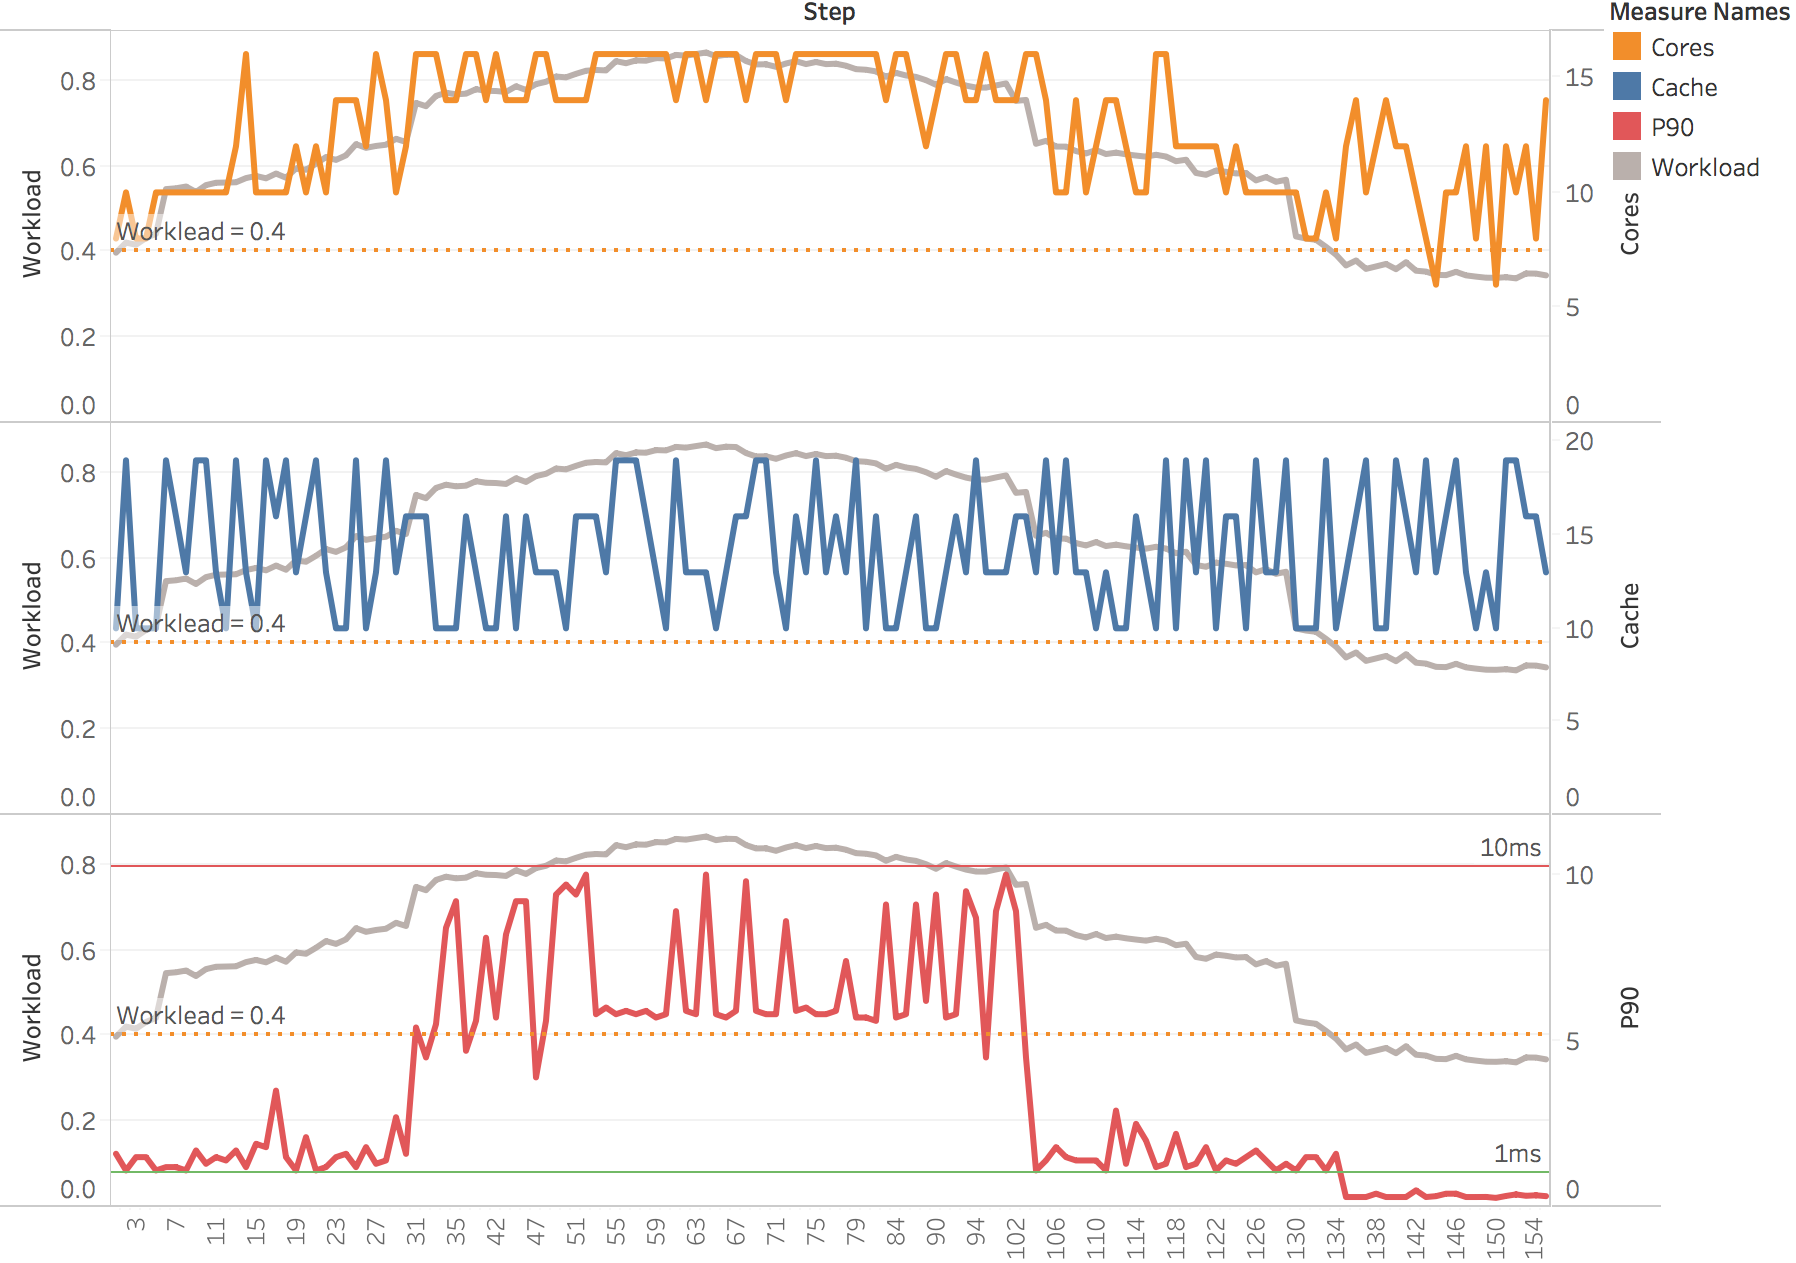
\includegraphics[width=1\linewidth]{result/run_example.png}
  \captionof{figure}{训练结果}
  \label{fig:actor_critic}
\end{figure}



